\documentclass[12pt]{article}
\usepackage[margin=8pt]{geometry}
\usepackage{tikz}
\usepackage{xcolor}
\usepackage{caption}
\usepackage[utf8]{inputenc}
\usepackage[T1]{fontenc}

% Times-like font, standard for journals
\usepackage{newtxtext,newtxmath}
\usepackage{microtype}

\usepackage{amsmath,amssymb}
\usepackage{graphicx}
\usepackage{stfloats}
\usepackage{booktabs}
\usepackage{caption}
\usepackage{subcaption}
\usepackage{float}
\usepackage{placeins}
\usepackage{adjustbox}
\captionsetup{justification=raggedright,singlelinecheck=false}
\captionsetup[subfigure]{labelformat=parens,labelsep=space}
\renewcommand\thesubfigure{\alph{subfigure}}
\usetikzlibrary{positioning,arrows,arrows.meta,shapes.geometric,shapes.misc}
\pagestyle{empty}
\raggedbottom
\begin{document}

\clearpage
\thispagestyle{empty}
\begin{center}
  \centering
  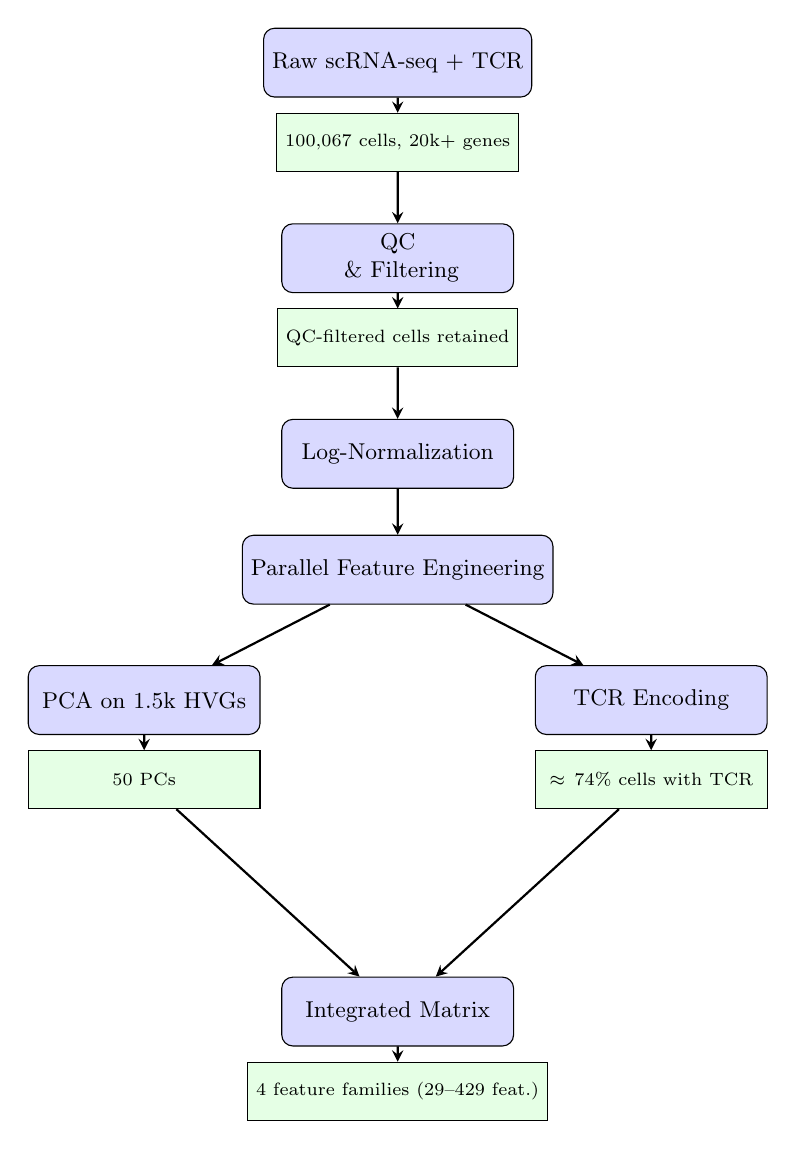
\begin{tikzpicture}[node distance=1.3cm, transform shape, scale=0.92]
    \tikzset{
      process/.style = {rectangle, rounded corners, minimum width=3.2cm, minimum height=0.95cm, align=center, draw=black, fill=blue!15, font=\small},
      data/.style = {rectangle, minimum width=3.2cm, minimum height=0.8cm, align=center, draw=black, fill=green!10, font=\scriptsize},
      arrow/.style = {thick,->,>=stealth}
    }
    
    \node (raw) [process] {Raw scRNA-seq + TCR};
    \node (raw_data) [data, below of=raw, yshift=0.2cm] {100,067 cells, 20k+ genes};
    \node (qc) [process, below of=raw_data, yshift=-0.3cm] {QC \\\ \& Filtering};
    \node (qc_data) [data, below of=qc, yshift=0.2cm] {QC-filtered cells retained};
    \node (norm) [process, below of=qc_data, yshift=-0.3cm] {Log-Normalization};
    \node (split) [process, below of=norm, yshift=-0.3cm] {Parallel Feature Engineering};
    
    \node (pca) [process, below of=split, xshift=-3.5cm, yshift=-0.5cm] {PCA on 1.5k HVGs};
    \node (pca_data) [data, below of=pca, yshift=0.2cm] {50 PCs};
    
    \node (tcr) [process, below of=split, xshift=3.5cm, yshift=-0.5cm] {TCR Encoding};
    \node (tcr_data) [data, below of=tcr, yshift=0.2cm] {$\approx\,74\%$ cells with TCR};
    
    \node (final) [process, below of=split, yshift=-4.8cm] {Integrated Matrix};
    \node (final_data) [data, below of=final, yshift=0.2cm] {4 feature families (29--429 feat.)};
    
    \draw [arrow] (raw) -- (raw_data);
    \draw [arrow] (raw_data) -- (qc);
    \draw [arrow] (qc) -- (qc_data);
    \draw [arrow] (qc_data) -- (norm);
    \draw [arrow] (norm) -- (split);
    \draw [arrow] (split) -- (pca);
    \draw [arrow] (split) -- (tcr);
    \draw [arrow] (pca) -- (pca_data);
    \draw [arrow] (tcr) -- (tcr_data);
    \draw [arrow] (pca_data) -- (final);
    \draw [arrow] (tcr_data) -- (final);
    \draw [arrow] (final) -- (final_data);
  \end{tikzpicture}
  \vspace{8pt}
  \captionof{figure}{Enhanced Data Processing Pipeline with quantitative details at each stage, showing cell counts, feature dimensions, and variance explained.}
\end{center}

\clearpage

\begin{figure}[htbp]
    \centering
    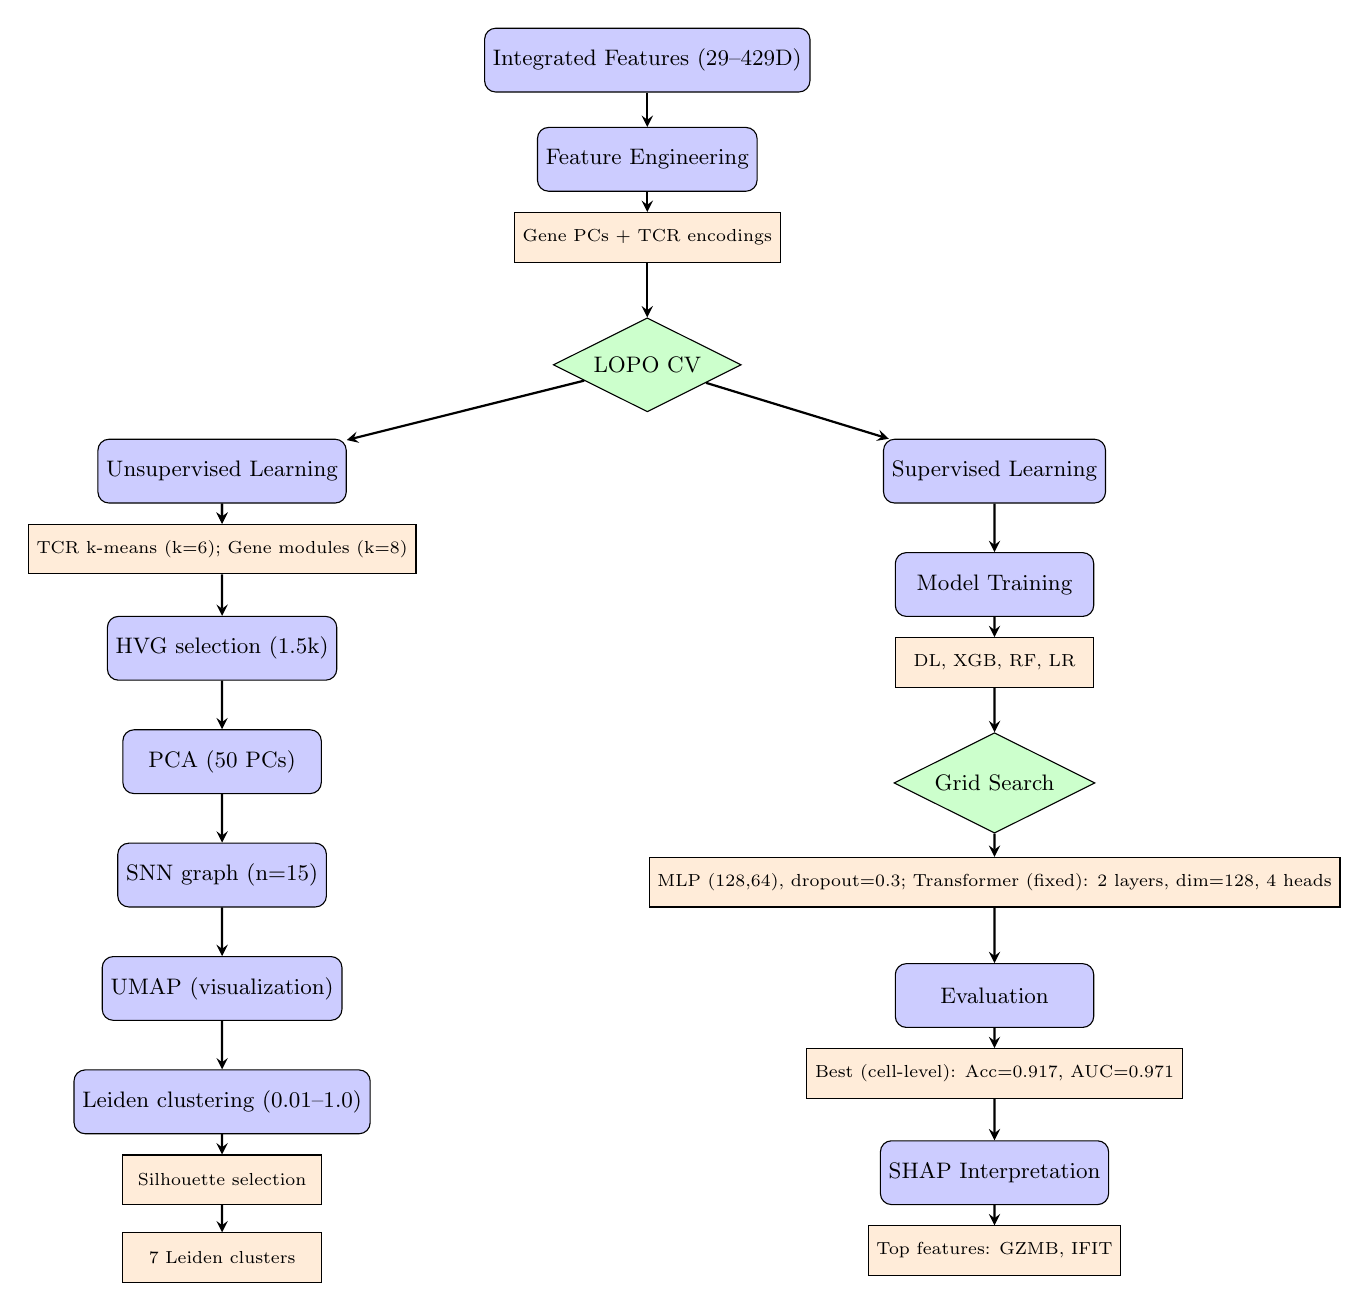
\begin{tikzpicture}[node distance=1.4cm, font=\small, transform shape, scale=0.9]
    \tikzset{
      process/.style = {rectangle, rounded corners, minimum width=2.8cm, minimum height=0.9cm, text centered, draw=black, fill=blue!20},
      decision/.style = {diamond, minimum width=2.2cm, minimum height=0.9cm, text centered, draw=black, fill=green!20, aspect=2},
      data/.style = {rectangle, minimum width=2.8cm, minimum height=0.7cm, text centered, draw=black, fill=orange!15, font=\scriptsize},
      arrow/.style = {thick,->,>=stealth}
    }
    
    \node (input) [process] {Integrated Features (29--429D)};
    \node (feat_eng) [process, below of=input] {Feature Engineering};
    \node (feat_data) [data, below of=feat_eng, yshift=0.3cm] {Gene PCs + TCR encodings};
    \node (split) [decision, below of=feat_data, yshift=-0.4cm] {LOPO CV};
    \node (unsup) [process, left of=split, xshift=-4.6cm, yshift=-1.5cm] {Unsupervised Learning};
    \node (tcr_kmeans) [data, below of=unsup, yshift=0.3cm] {TCR k-means (k=6); Gene modules (k=8)};
    \node (hvg) [process, below of=tcr_kmeans, yshift=0cm] {HVG selection (1.5k)};
    \node (pca_unsup) [process, below of=hvg, yshift=-0.2cm] {PCA (50 PCs)};
    \node (snn) [process, below of=pca_unsup, yshift=-0.2cm] {SNN graph (n=15)};
    \node (umap) [process, below of=snn, yshift=-0.2cm] {UMAP (visualization)};
    \node (leiden) [process, below of=umap, yshift=-0.2cm] {Leiden clustering (0.01--1.0)};
    \node (silhouette) [data, below of=leiden, yshift=0.3cm] {Silhouette selection};
    \node (unsup_data) [data, below of=silhouette, yshift=0.3cm] {7 Leiden clusters};
    \node (sup) [process, right of=split, xshift=3.5cm, yshift=-1.5cm] {Supervised Learning};
    \node (train) [process, below of=sup, yshift=-0.2cm] {Model Training};
    \node (train_data) [data, below of=train, yshift=0.3cm] {DL, XGB, RF, LR};
    \node (tune) [decision, below of=train_data, yshift=-0.3cm] {Grid Search};
    \node (tune_data) [data, below of=tune, yshift=0cm] {MLP (128,64), dropout=0.3; Transformer (fixed): 2 layers, dim=128, 4 heads};
    \node (eval) [process, below of=tune_data, yshift=-0.2cm] {Evaluation};
    \node (eval_data) [data, below of=eval, yshift=0.3cm] {Best (cell-level): Acc=0.917, AUC=0.971};
    \node (interpret) [process, below of=eval_data, yshift=0cm] {SHAP Interpretation};
    \node (interpret_data) [data, below of=interpret, yshift=0.3cm] {Top features: GZMB, IFIT};
    
    \draw [arrow] (input) -- (feat_eng);
    \draw [arrow] (feat_eng) -- (feat_data);
    \draw [arrow] (feat_data) -- (split);
    \draw [arrow] (split) -- (unsup);
    \draw [arrow] (unsup) -- (tcr_kmeans);
    \draw [arrow] (tcr_kmeans) -- (hvg);
    \draw [arrow] (hvg) -- (pca_unsup);
    \draw [arrow] (pca_unsup) -- (snn);
    \draw [arrow] (snn) -- (umap);
    \draw [arrow] (umap) -- (leiden);
    \draw [arrow] (leiden) -- (silhouette);
    \draw [arrow] (silhouette) -- (unsup_data);
    \draw [arrow] (unsup) -- (tcr_kmeans);
    \draw [arrow] (split) -- (sup);
    \draw [arrow] (sup) -- (train);
    \draw [arrow] (train) -- (train_data);
    \draw [arrow] (train_data) -- (tune);
    \draw [arrow] (tune) -- (tune_data);
    \draw [arrow] (tune_data) -- (eval);
    \draw [arrow] (eval) -- (eval_data);
    \draw [arrow] (eval_data) -- (interpret);
    \draw [arrow] (interpret) -- (interpret_data);
    \end{tikzpicture}
    \captionof{figure}{Enhanced Modeling Pipeline: Two-stage strategy with feature engineering, hyperparameter optimization via grid/randomized search, and LOPO cross-validation. Representative deep model hyperparameters (MLP selected via inner CV; CNN/BiLSTM/Transformer used fixed representative configurations) and Leiden clustering outputs (target: 7~clusters, silhouette-optimized resolution) are shown.}
\end{figure}

\FloatBarrier

\begin{figure}[htbp]
  \centering
  \begin{subfigure}[b]{0.92\linewidth}
    \centering
    \adjustbox{max size={\linewidth}{\dimexpr0.45\textheight-15pt\relax}}{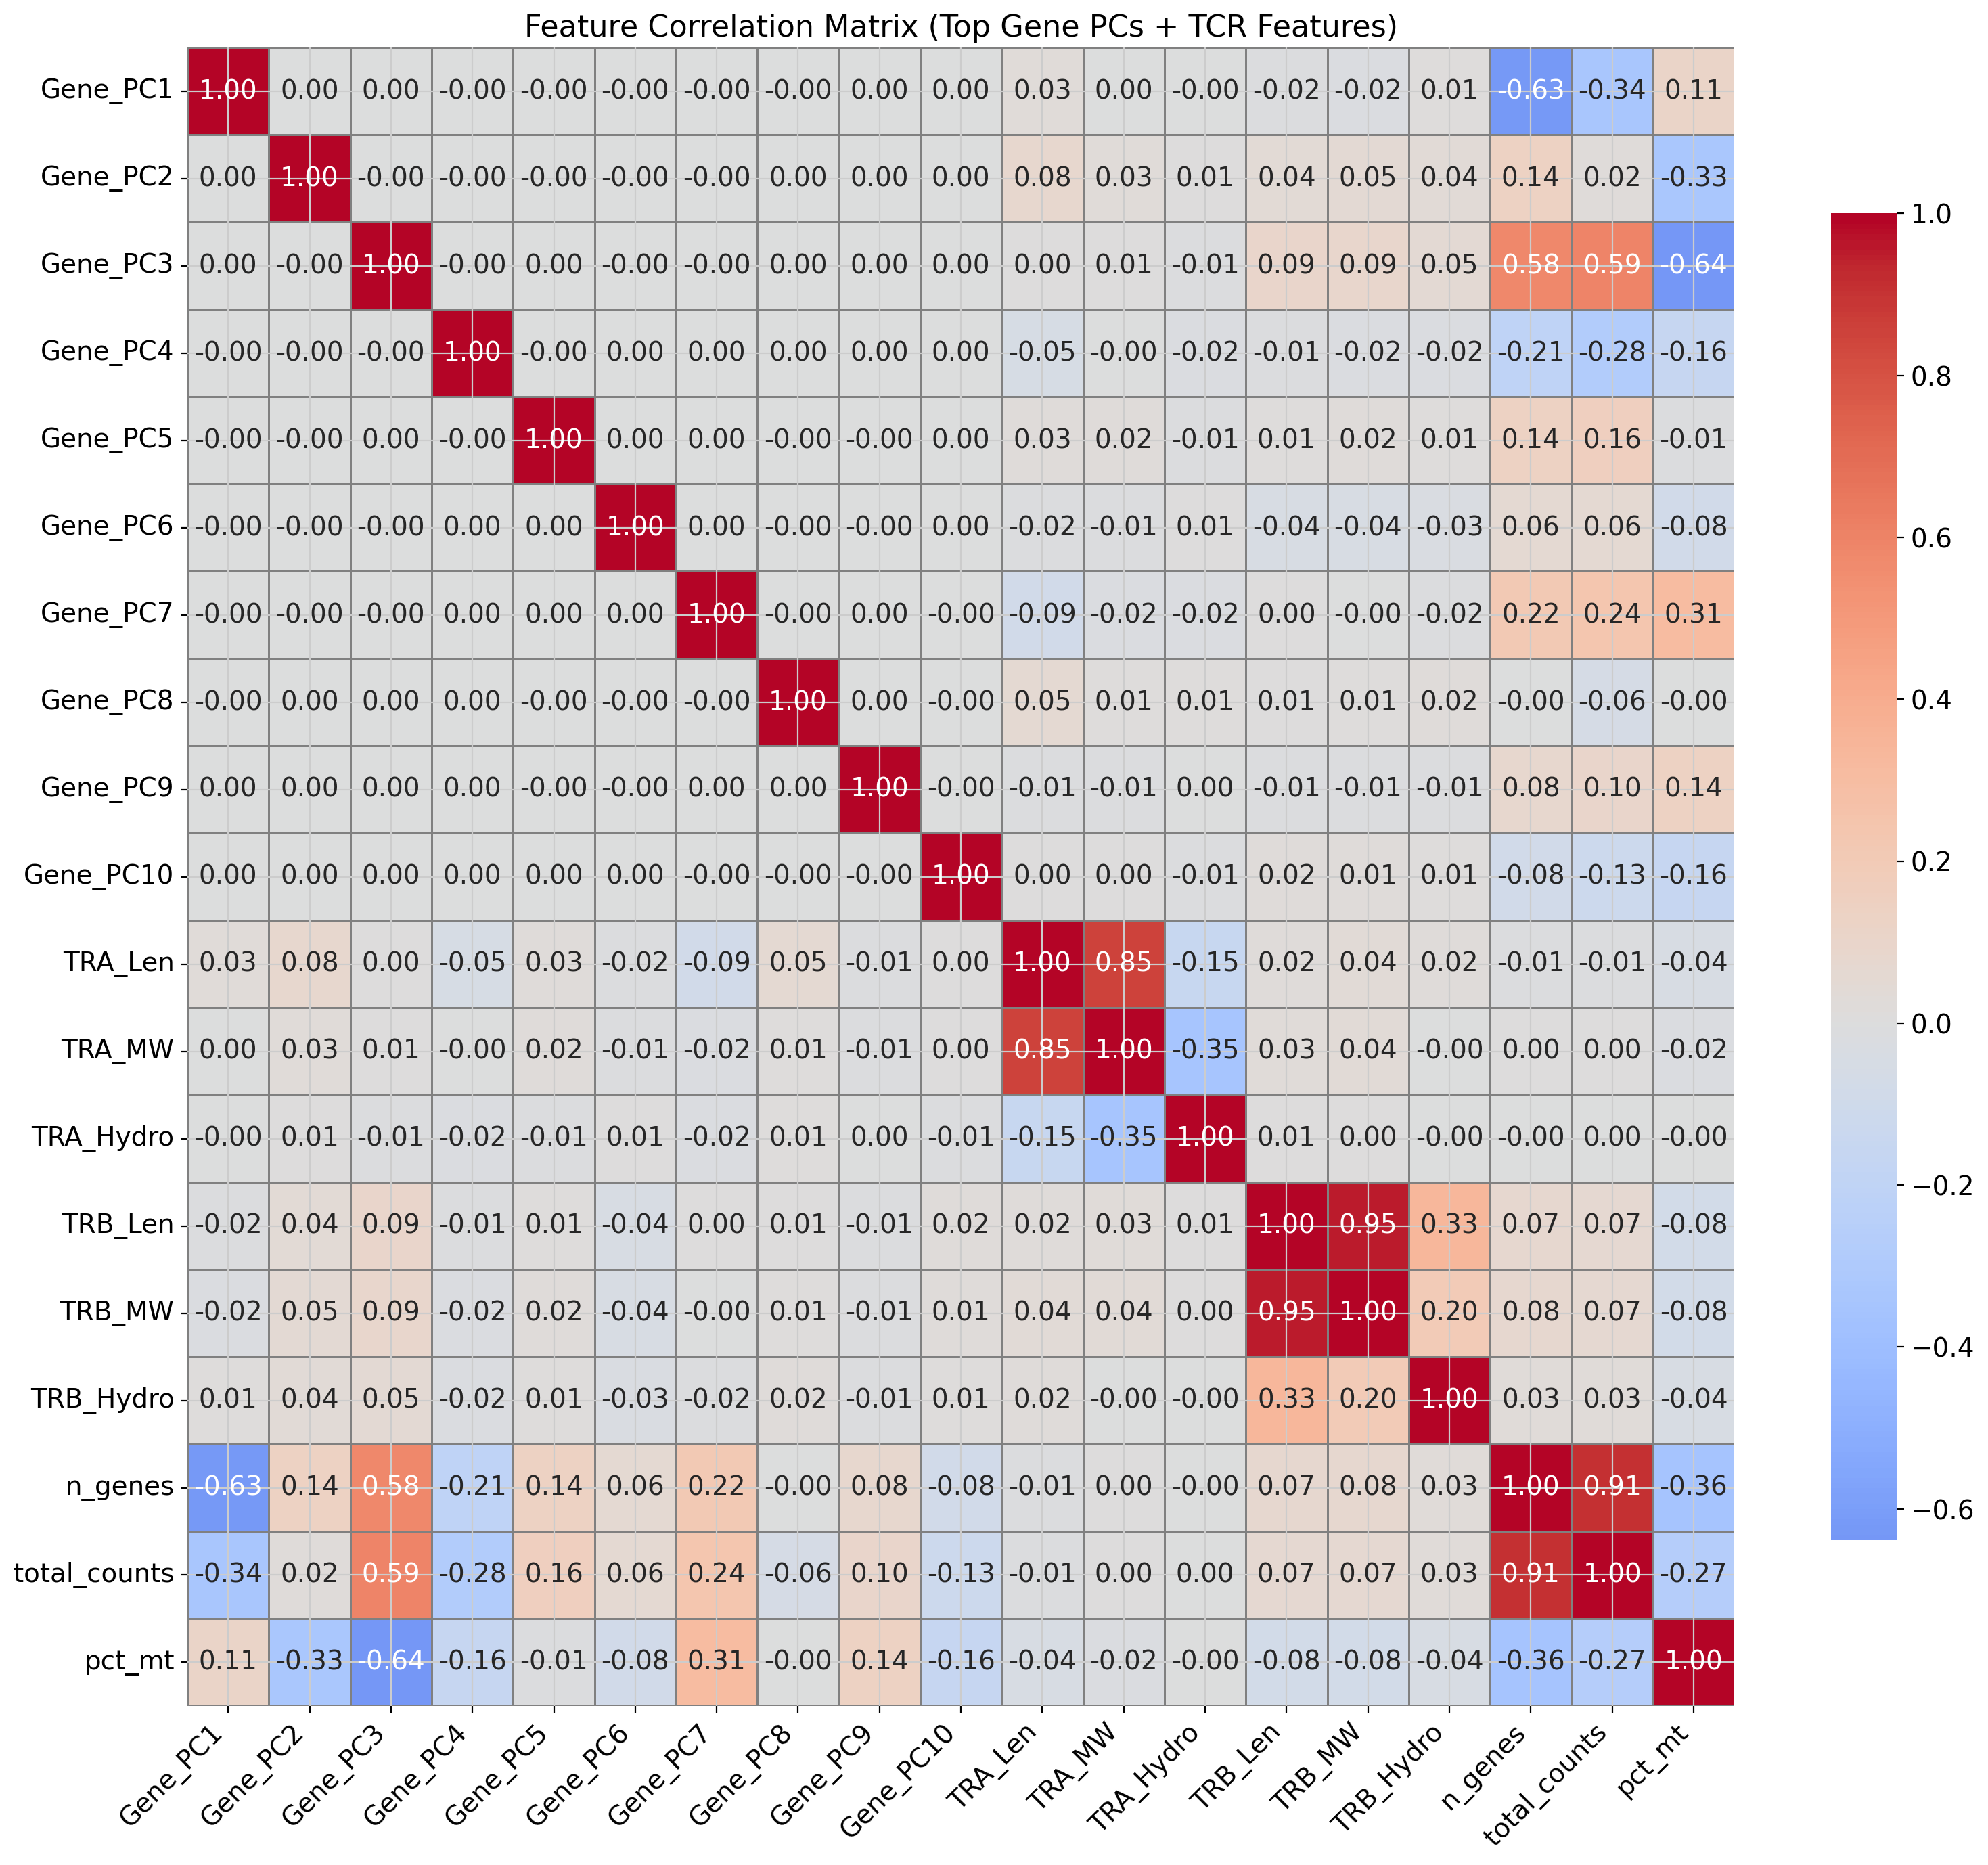
\includegraphics{Feature_Heatmappng.png}}
    \caption{Heatmap of the correlation matrix for the top engineered features (first 20 PCs and select receptor summaries).}
  \end{subfigure}
  \vspace{8pt}
  \begin{subfigure}[b]{0.92\linewidth}
    \centering
    \adjustbox{max size={\linewidth}{\dimexpr0.45\textheight-15pt\relax}}{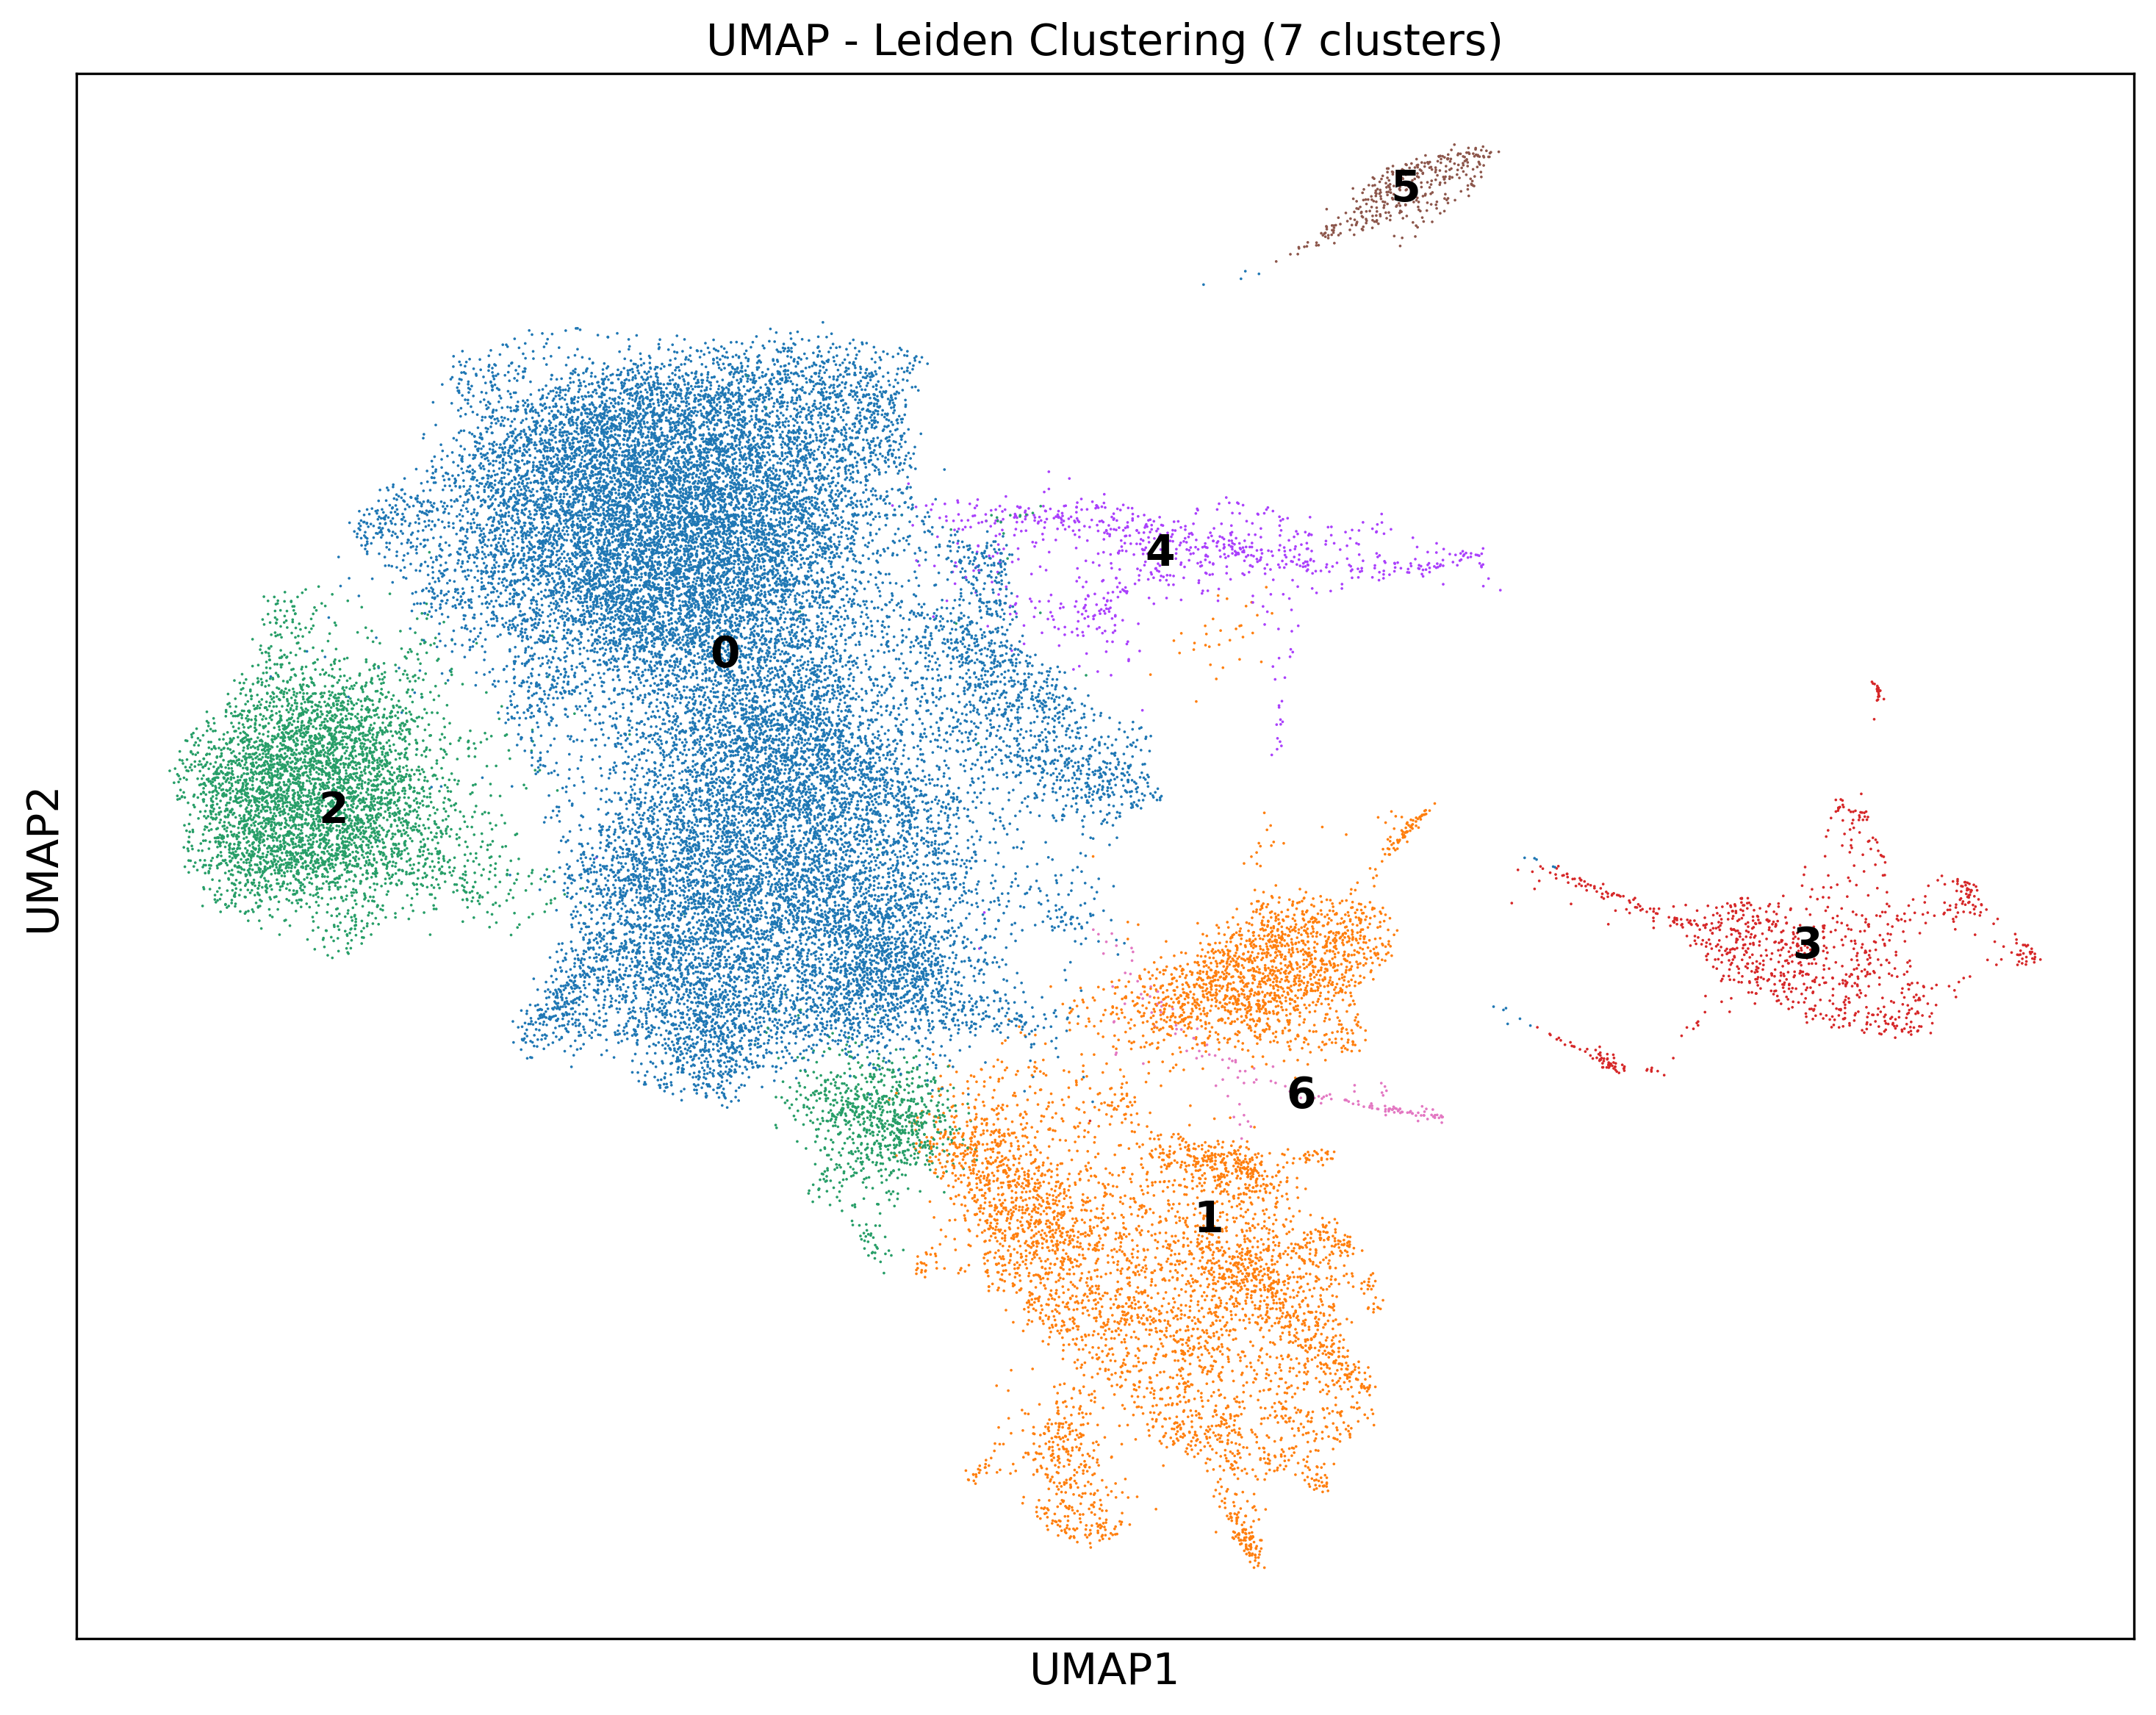
\includegraphics{umap_clusters.png}}
    \caption{UMAP visualization of Leiden clusters colored by cluster assignment.}
  \end{subfigure}
  \vspace{6pt}
  \caption{Heatmap and UMAP visualization of engineered features and clusters.}
\end{figure}
\end{document}